\section{Makanya}

\subsection{Hintergrund} % Makanya
Der Hintergrund des Makanya.com Projektes ist eine Partnerschaft
zwischen der Kirchengemeinde Kühlungsborn und Tansania,
sowie der Partnerschaft zwischen der Kirchengemeinde und dem Schulzentrum Kühlungsborns.
Der Pastor Kühlungsborns, Matthias Borchert,
suchte den Kontakt zum \jf Team über das Schulzentrum.
Nach einer kurzen Bekanntmachung durch Frau Schmidt war die Zusammenarbeit besiegelt.\\
Eine Domain (\link{makanya.com}) von strato.de war bereits vorhanden% TODO Quelle + Preise
% Server: strato.de
und ein WordPress Blog \link{kulungsi.com}.
Die Website musste technisch aufbereitet werden, und eine englische Übersetzung war notwendig.
Diese Website sollte dann als Anlaufpunkt für alle Projektteilnehmer, Interessenten und Schüler sein.
% Sprache: Deutsch, Englisch, Zusammenarbeit (Dolmetschering: Frau Wieck)
Aus dieser Spezifizierung ergeben sich die Anforderungen an die Programmierung:\\
Der Inhalt der Website muss auf Deutsch und Englisch sein, beide Versionen weitestgehend identisch.
Weiterhin soll die Webseite einfach bedienbar sein,
damit auch technisch unbegabte Schüler und Verwaltungsmitglieder sich durch die Webseite navigieren können sollen.
Damit die Seite auch in Tansania erreichbar ist müssen die Datenformate optimiert werden.\\
% Programmierung: PHP, HTML, MySQL
% Mehr Programmierung...?
% Beiprogramm: Schulzentrum -> Spendenlauf, Besuch der Tansanianer, Meetings, Auswertung
Somit stellt diese Arbeit ein Teil eines größeren Projektes dar.
Dieses Projekt beinhaltet die Partnerschaft von der Kirchengemeinde mit dem Schulzentrum und Makanya in Tansania.
Andere Aspekte beinhalten den Schüleraustausch und Besuch der Tansanianer,
sowie ein von der Schule organisierter Spendenlauf der die Finanzierung des Fluges ermöglichte.

\subsection{Methodik} % Makanya
% Aufteilung:
% Markus: Programmierung, Öffentlichkeitsarbeit, Infos

% Umgebung: Sublime Text, PHPmyAdmin,
% Hilfe: php.net (erstes PHP Projekt)
% Sicherheit: sha256 Schlüssel, TODO Vortrag herauskramen!
Die hauptsächliche Arbeit wurde in der Programmiersprache PHP erledigt.
Da das Ergebnis als Website erreichbar sein sollte,
war von Anfang an klar, dass die Seite am Ende den Nutzer in HTML, CSS und JavaScript
erreichen müsse.
Die Programmierung des Backends geschah in Kürze nach dem ersten Treffen und der Übergabe der Logindaten.
Die Website war funktionsfähig sobald sie die Informationen auf Kulungsi.com widerspiegelte.
Da dieses Ziel schnell erreicht war, sollte nun weiterführend eine Art soziales Netzwerk zwecks Austausch im Hintergrund errichtet werden.
Dieser Teil der Website ist zum Zeitpunkt der Setzung noch nicht fertiggestellt, die grundlegenden
Funktionen: Chats, Accounts, Gruppen und weitere Kleinigkeiten sind allerdings schon funktionstüchtig.\\
Die Entwicklung wurde durch den Texteditor Sublime Text erleichtert. Als Testserver diente ein von mir sonst privat genutzter Raspberry Pi,
wobei ich allerdings von vornherein auf der von Strato.de zur Verfügung gestellten Datenbank arbeitete.
Außerdem hervorstechend ist das erste größere Treffen des Tansaniakreises Kühlungsborns, dem ich beiwohnte.
Meine Aufgabe war es dem Kern der Gemeinde meine Fortschritte zu präsentieren.
Eine Präsentation mit für diesen Anlass erzeugten Grafiken diente um die Entwicklung einer Website
sowie die damit verbundenen Schwierigkeiten, Limitationen und Abläufe visuell zu erläutern.


\subsection{Ergebnis} % Makanya
Das Ergebnis dieses Projektes ins die Webseite, die statische Informationen über Makanya bereitstellt.
Dazu gibt es im Hintergrund eine minimale Version eines sozialen Netzwerkes mit einem offenen und geschlossenen Chat.
Außerdem wurden alle von dem Projekt erwarteten Sicherheitsbedingungen eingehalten.
Auf der Sicherheit liegt bis heute noch der Fokus:
solange die Website erreichbar ist und die richtigen Informationen anzeigt ist ihre Aufgabe erfüllt.
Die Autoritätspersonen und Lehrer bekamen außerdem die Möglichkeit die ihnen untergestellten Schüler zu verwalten.
Somit konnte auch die Idee des Konten- und Rechtssystems umgesetzt werden.\\
Da dieses Teilgebiet der Arbeit nicht viel Beaufsichtigung und stetige Entwicklung verlangt ist
es im Verlauf der Arbeit auf der Prioritäten-liste langsam abgestiegen.
\begin{center}
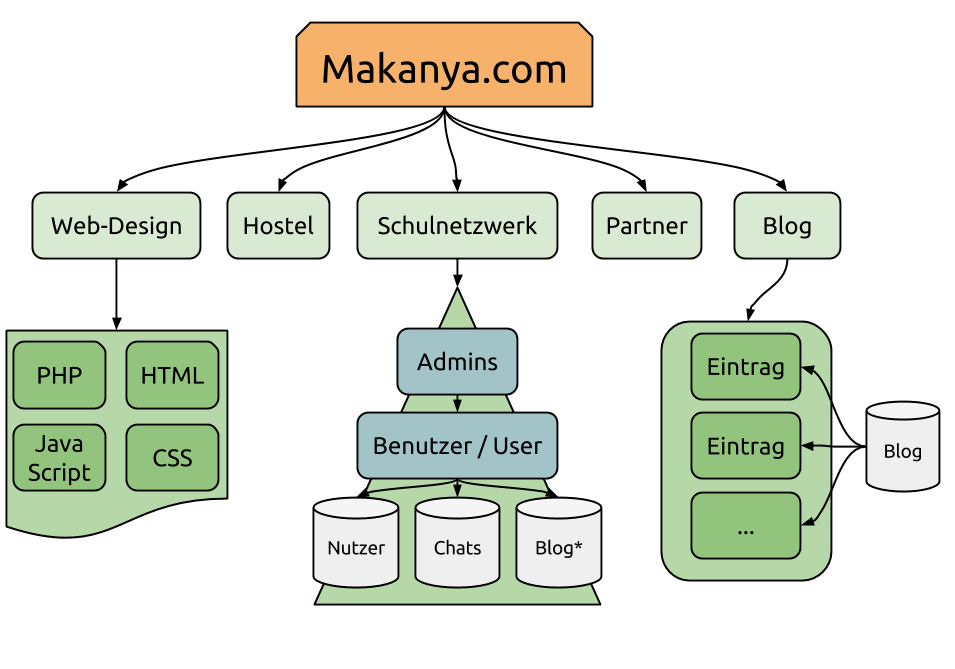
\includegraphics[width=\linewidth]{imgs/makanyaOverview.png}
\end{center}
